\documentclass[tikz,crop]{standalone}
\begin{document}
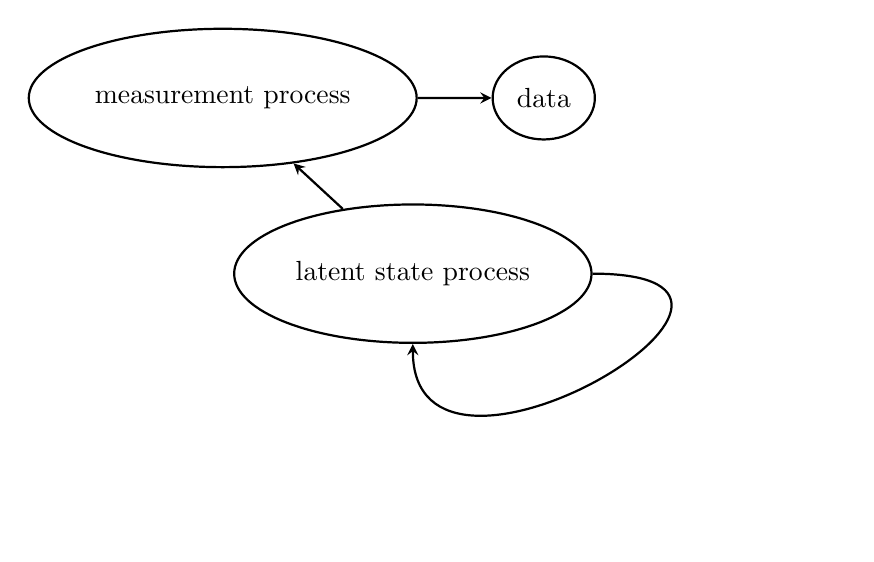
\begin{tikzpicture}[scale=0.8]
  \usetikzlibrary{shapes,arrows.meta,positioning,calc}

  \tikzstyle{coordinate}=[inner sep=0pt,outer sep=0pt]
  \tikzstyle{concept}=[shape=ellipse, color=black, draw, fill=white, thick, minimum height=3em]
  \tikzstyle{connection}=[color=black, thick, >=stealth]

  \node [concept,minimum height=5em] (X) at (0,0) {latent state process};
  \node [concept,minimum height=5em] (Y) at ($(X.north west)+(-1,2)$) {measurement process};
  \node [concept] (D) at ($(Y.east)+(2,0)$) {data};
  \draw[connection,->] (X) -- (Y);
  \draw[connection,->] (Y) -- (D);
  \draw[connection,->] (X.east) .. controls ($(X.east)+(0:4)$) and ($(X.south)+(-90:3)$) .. (X.south);
\end{tikzpicture}
\end{document}
